\documentclass{article}

\usepackage{url}
\usepackage{amsmath,amssymb}
\usepackage{graphicx,svg}

\begin{document}
\title{Lecture 6\\ Complex Analysis I}
\author{C.L. Wyatt}
\date{\today}
\maketitle

The primary tools we will develop in this course are the Laplace and Z-transform. Because the inverse of these transforms is an integral in the complex plane, it is helpful to have a basic understanding of complex analysis. Over the next three lectures we will introduce the concepts and methods of complex analysis. Today we will review complex numbers and complex functions $f: \mathbb{C} \rightarrow \mathbb{C}$.

\section{Complex Numbers}

Recall the basics of complex numbers

\begin{itemize}
\item $j$ is the imaginary unit, the solution to $s^2 + 1 = 0$, $j = \sqrt{-1}$.
\item a complex number is the combination of two real numbers $x,y$ with the imaginary unit using addition and multiplication $s = x + j\, y$
\item we write $s\in\mathbb{C}$
\item $x = \text{Re}(s)$ is the real part of $s$
\item $y = \text{Im}(s)$ is the imaginary part of $s$
\item if $x=0$ $s$ is purely imaginary, if $x=0$ $s$ is purely real, note $s = 0+j0 = 0$ is the only complex number that is both
\item given two complex numbers $s_1 = x_1 + jy_1$ and $s_2 = x_2 + jy_2$
  \begin{itemize}
  \item they are equal if and only if $x_1 = x_2$ and $y_1 = y_2$
  \item $s_1 + s_2 = (x_1 + x_2) + j(y_1 + y_2)$
  \item $s_, s_2 = (x_1 + jy_1)(x_2 + jy_2) = (x_1x_2 - y_1y_2) + j(x_1y_2 + x_2y_1)$
  \item $\frac{s_1}{s_2}$, $s_2 \neq 0$ can be expressed as
    \begin{align}
      \frac{s_1}{s_2} &= \frac{x_1 + jy_1}{x_2 + jy_2}\\
      &= \frac{x_1 + jy_1}{x_2 + jy_2}\cdot \frac{x_2 - jy_2}{x_2 - jy_2}\\
      &= \frac{(x_1x_2 + y_1y_2) + j(x_2y_1 - x_1y_2)}{x_2^2 + y_2^2} 
    \end{align}
  \end{itemize}
\item $s^* = x - jy$ is the conjugate of $s = x+jy$
\item $|s| \geq 0$ is the absolute value or modulus
  \[
  |s| = |a +jy| = \sqrt{x^2 + y^2} = \sqrt{s\, s^*}
  \]
\end{itemize}

Some properties of complex numbers that are often useful:

\begin{itemize}
\item $| s_1 \cdot s_2 \cdots s_n| = | s_1| \cdot |s_2| \cdots |s_n|$
\item $\left| \frac{s_1}{s_2} \right| = \frac{|s_1|}{|s_2|}$
\item note that $|s_1 + s_2| \neq |s_1| + |s_2|$, a common mistake
\item the real and imaginary part of a complex number $s$ can be expressed as
  \begin{align}
    \text{Re}(s) = \frac{s+s^*}{2}\\
    \text{Im}(s) = \frac{s-s^*}{2j}
  \end{align}
\item the conjugate of the sum/product/ratio is the sum/product/ratio of the conjugates
  \begin{align}
    (s_1 + s_2)^* &= s_1^* + s_2^*\\
    (s_1 \cdot s_2)^* &= s_1^* \cdot s_2^*\\
    \left(\frac{s_1}{s_2}\right)^*, \, s_2 \neq 0 &= \frac{s_1^*}{s_2^*} 
  \end{align}
\item inequalities

  \begin{align}
    -|s| \leq \text{Re}(s) \leq |s|\\
    -|s| \leq \text{Im}(s) \leq |s|\\
    |s_1 + s_2| \leq |s_1| + |s_2|\\
    |s_1 + s_2 + \cdots s_n| \leq |s_1| + |s_2| + \cdots |s_n|\\
  \end{align}
\end{itemize}

\subsection{Geometric Representation of the Complex Plane}

A complex number is a two-dimensional vector in the complex plane

\begin{figure}
  \centering
  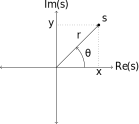
\includegraphics[alt={a complex number in the complex plane}]{fig6_1.svg}
\end{figure}

where

\begin{itemize}
\item $r = |s|$ is variously the norm, length, modulus, magnitude
\item $\theta = \tan^{-1}\left(\frac{y}{x}\right) $ is variously the angle, argument, or phase
\item $x = r\cos(\theta)$ is the real part
\item $y = r\sin(\theta)$ is the imaginary part
\end{itemize}

In cartesian form
\begin{align}
  s &= x + jy\\
  &= r\cos(\theta) + jrsin(\theta)\\
  &= r\left[ \cos(\theta) + j\sin(\theta)\right]
\end{align}

In polar form

\[
s = r e^{j\theta}
\]

Equating the two forms we can see Euler's identity
\[
s = r e^{j\theta} = r\left[ \underbrace{\cos(\theta) + j\sin(\theta)}_{\text{Euler's identity}}\right]
\]

and some commonly used manipulations:

\begin{itemize}
\item $s_1 \cdot s_2 = r_1 e^{j\theta_1} \cdot r_2 e^{j\theta_2} = r_1 \cdot r_2 e^{j(\theta_1 + \theta_2)} = r_1 r_2\left[\cos(\theta_1 + \theta_2) + j\sin(\theta_1 + \theta_2)\right]$
\item $|s| = |r e^{j\theta}| = |r||e^{j\theta}| = r$
\item $\cos(\theta) = \frac{1}{2}e^{j\theta} + \frac{1}{2}e^{-j\theta}$
\item $\sin(\theta) = \frac{1}{2j}e^{j\theta}  \frac{1}{2j}e^{-j\theta}$
\end{itemize}

Note that the complex plane is a vector space spanned by the real and imaginary part. Any vector in the space rotated by $2\pi$ is indistinguishable from any other, i.e. $r e^{j\theta} = re^{j(\theta + 2\pi n)}$ for any $n\in\mathbb{Z}$. When $n = 0$ $\theta = \theta_p$ is called the principle argument.

\section{Complex Valued Functions}

You should be already very familiar with complex valued functions from ECE 2714, as they are used extensively: $f: \mathbb{R} \rightarrow \mathbb{C}$. Some properties

\begin{align}
  f(t) &= x(t) + jy(t)\\
  \frac{df}{dt} &= \frac{dx}{dt} + j\frac{dy}{dt}\\
  \int f(t)\; dt &= \int x(t)\; dt + j\int y(t)\; dt + C
\end{align}

Examples are time domain functions, e.g.

\[
e^{j\omega t} = cos(\omega t) + j\sin(\omega t)
\]

and frequency domain functions, e.g.

\[
H(\omega) = \frac{1}{1+j\omega}
\]

\section{Complex Functions}

We now focus on the functions we will be studying for much of the semester, complex functions or complex-valued functions onf a complex argument $f: \mathbb{C} \rightarrow \mathbb{C}$. Following our notation above where $s = x + jy$, we write

\[
f(s) = \underbrace{u(x,y)}_{\text{Re}(s)} + j \underbrace{v(x,y)}_{\text{Im}(s)}
\]
where the real and imaginary parts of $f(s)$ are functions $u,v$ from $\mathbb{R}^2$ onto $\mathbb{R}$. In other words, the real part of $f(s)$ is a function of the real \textbf{and} imaginary parts of $s$, and the imaginary part of $f(s)$ is also a function of the real \textbf{and} imaginary parts of $s$.

Some examples. Note in some cases the cartesian form is preferred while in others the polar form is clearer.

\begin{itemize}
\item $f(s) = s = \text{Re}(s) + j\text{Im}(s)$
\item $f(s) = s^* = \text{Re}(s) - j\text{Im}(s)$
\item $f(s) = s^2 = \left(re^{j\theta}\right)^2 = r^2 e^{j2\theta}$
\item $f(s) = s^n$ for $n\in\mathbb{Z}$
\item polynomials: $f(s) = \sum\limits_{k = 0}^N a_ks^k$
\item power series expansion about $s_0$: $f(s) = \sum\limits_{k = 0}^N (s-s_0)^k$
\item rational functions
  \[
  f(s) = \frac{\sum\limits_{k = 0}^M a_ks^k}{\sum\limits_{k = 0}^N a_ks^k}
  \]
\end{itemize}

The last example will be particularly important as the system function for LTI systems is a rational function in most cases.

The previous examples were all single-valued functions. Lets look at two interesting multi-valued functions.

\begin{itemize}
\item You know that for $x\in\mathbb{R}$ the solution to $x^2 = y$ is $\pm \sqrt{y}$, the function is mult-valued. Similarly for complex numbers (derivation omitted)

  \[
  \sqrt{s} = \sqrt{x + jy} = \pm \left[\sqrt{\frac{x + \sqrt{x^2 + y^2}}{2}} + j\frac{y}{|y|} \sqrt{\frac{-x + \sqrt{x^2 + y^2}}{2}}\right] 
  \]
  if $y \neq 0$. If $y = 0$ then
  \[
  \sqrt{s} = \sqrt{x} = \pm \sqrt{|x|}
  \]
  
\item Another example is the inverse of $e^s$m $\ln(s)$
  \[
  \ln(s) = \ln(|s|) + j(\theta_p + 2\pi n)  
  \]
  where $n\in\mathbb{Z}$ and $\theta_p$ is the principle argument.
\end{itemize}

\subsection{Visualizing Complex Functions}

Since the argument to a complex function is a pair of real numbers and the resulting value is also a pair, we have to use surface or contour plots to visualize complex functions.

Using surface plots we need two, for the real part and imaginary part of the function value or for the magnitude and phase of the function value. For example consider the complex function

\[
f(s) = f(x + jy) = x^2\cdot y + jx\cdot y
\]

\begin{figure}
  \centering
  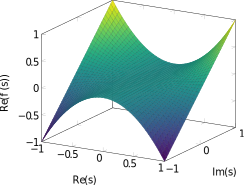
\includegraphics[alt={a surface plot of real part for the example}]{fig6_2.svg}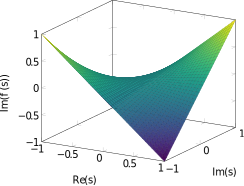
\includegraphics[alt={a surface plot of imaginary part for the example}]{fig6_3.svg}
  \caption{Surface plot of real and imaginary part for the example.}
\end{figure}

\begin{figure}
  \centering
  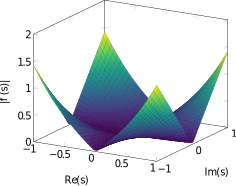
\includegraphics[alt={a surface plot of magnitude for the example}]{fig6_4.svg}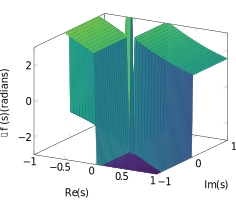
\includegraphics[alt={a surface plot of phase for the example}]{fig6_5.svg}
  \caption{Surface plot of magnitude and phase for the example.}
\end{figure}

For contour plots we again need two plots, either for the real part and imaginary part or for the magnitude and phase. However theses plots consist of a set of curves each defining an iso-contour, all the points whose function value takes on a constant. These are essential topographical maps.

\begin{figure}
  \centering
  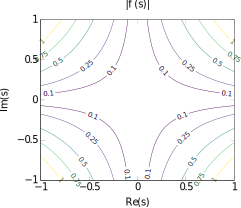
\includegraphics[alt={a contour plot of magnitude for the example}]{fig6_6.svg}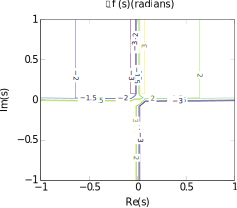
\includegraphics[alt={a contour plot of phase for the example}]{fig6_7.svg}
  \caption{Coutour plot of magnitude and phase for the example.}
\end{figure}


\subsection{Limits of Complex Functions}

Recall from your first calculus course the definition of a limit for functions $f:\mathbb{R}\rightarrow\mathbb{R}$. The limit of a function at a domain value $x_0\in\mathbb{R}$, written as

\[
\lim_{x \rightarrow x_0} f(x) = y_0 
\]
exists if for some $\epsilon > 0$, there exists a $\delta > 0$ such that
$0 < |x-x_0| < delta$ implies $|f(x) - y_0| < \epsilon$.

Similarly for complex functions $g:\mathbb{C}\rightarrow\mathbb{C}$, the 
limit of a function at a complex value in the domain $s_0\in\mathbb{C}$, written as

\[
\lim_{s \rightarrow s_0} f(s) = w 
\]
exists if for some $\epsilon > 0$, there exists a $\delta > 0$ such that
$0 < |s-s_0| < \delta$ implies $|f(s) - w| < \epsilon$. However we can approach $s_0$ from any direction.

\begin{figure}
  \centering
  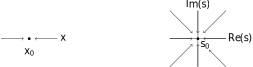
\includegraphics[alt={approaching a point on the real line contrasted with approaching a point in the complex plane}]{fig6_8.svg}
\end{figure}

We will use the concept of a limit to define the derivative of a complex function at our next meeting.

\subsection{Point at Infinity}

In calculus it is often useful to extend the real line to include $\pm\infty$, often denoted $\mathbb{R}^* = \mathbb{R} \cup \{-\infty, \infty\}$. However because the complex plane $\mathbb{C}$ has no ordering (it is a 2D vector space) there is only one point at infinity and $\mathbb{C}^* = \mathbb{C} \cup \{\infty\}$, where for $s\in\mathbb{C}$

\begin{itemize}
\item $s + \infty = \infty$
\item $s \cdot \infty = \infty$
\item $\infty + \infty = \infty$
\item $\infty \cdot \infty = \infty$
\item $\frac{s}{\infty} = 0$
\end{itemize}

and $\frac{\infty}{\infty}, 0\cdot\infty, \infty-\infty$ are undefined.

To visualize the extended complex plane, $\mathbb{C}^*$, we can use the Riemann sphere.

\begin{figure}
  \centering
  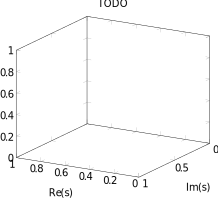
\includegraphics[width=0.5\linewidth, alt={the Riemann sphere and the orthographic prjection of a point in the complex plane}]{fig6_9.svg}
  \caption{FIGURE TODO.}
\end{figure}

In the above figure the line from a pont $s$ to $(0,0,1)$ intersects the sphere at some point $(x_0,y_0,z_0)$ where $s = \frac{x_0 + jy_0}{1-z_0}$ (stereographic projection). In this view the point $s = \infty$ corresponds to the point $(0,0,1)$.

\subsection{Curves in the Complex Plane}

Another concept that we will use extensively is that of curves in the complex plane. Let $p$ be a parameterization of a curve in $\mathbb{C}$. A curve is defined as $C = s(p) = x(p) _ jy(p)$ for $a \leq p \leq b$. The point $s_0 = s(a) = x(a) + jy(a)$ is the initial point. The point $s_1 = s(b) = x(b) + jy(b)$ is the terminal or final point.

\begin{figure}
  \centering
  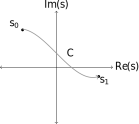
\includegraphics[alt={a smooth curve joining two points in the complex plane}]{fig6_10.svg}
\end{figure}

\begin{itemize}
\item If $s_0 = s_1$, then the curve is \textit{closed}.
\item The curve is \textit{smooth} if
  \[
  \frac{ds}{dp} = \frac{dx}{dp} + j \frac{dy}{dp} 
  \]
  is continuous and never zero for $a \leq p \leq b$ (the curve must change in some direction).
\item The curve is piece-wise smooth if it is smooth except at a finite number of points which join.
  
\begin{figure}
  \centering
  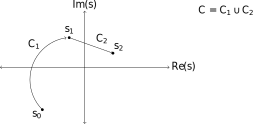
\includegraphics[alt={of two curves joined together into a disjpint but continuous curve}]{fig6_11.svg}
\end{figure}

\item The curve is simple if $s(p_1) \neq s(p_2)$ for $p_1 \neq p_2$ except possibly $p_1=a$, $p_2 = b$ and the curve is closed. This means that there are no sef-intersections. 
\end{itemize}

We will use curves to define contour integration of complex functions in future meetings.


\end{document}
